\documentclass[conference,10pt]{IEEEtran}
\IEEEoverridecommandlockouts
\usepackage[T1]{fontenc}
\usepackage[utf8]{inputenc}
\usepackage{cite}
\usepackage{microtype}
\usepackage{amsmath}
\usepackage{graphicx}
\usepackage{booktabs}
\usepackage{tabularx}
\usepackage{array}
\usepackage{xcolor}
\usepackage{tikz}
\usetikzlibrary{positioning,shapes.geometric,arrows.meta,calc}
\usepackage[hidelinks]{hyperref}

\newcommand{\cc}[1]{\texttt{#1}}

\begin{document}

\title{Concerns, Not Bugs: A Design-Based Study of\\Where Research Code Asks for Trust}

\author{\IEEEauthorblockN{Julian Dehne}
\IEEEauthorblockA{Research Software Engineering\\
Gesellschaft f\"ur Informatik e.V. (GI)\\
Berlin, Germany\\
\texttt{[email]}}}

\maketitle

\begin{abstract}
A research result can be wrong although every test passes: an unrecorded seed, a drifting language model, a silent record filter. We call such places \emph{concerns}: trust risks rather than bugs. Following design-based research, we report two design cycles of \texttt{rse\_annotations}, a Python tool in which authors mark concerns with decorators, a static scan detects unmarked candidates, and a reviewer inspects each marked place against the concern's assertion. Each concern is motivated by documented failures in the reproducibility literature. Checks are organised along two distinctions, detected versus declared and static versus runtime, which yield four quadrants. We model the inspection process as a UML activity diagram. In a research pipeline of 254 functions, only 2\,\% were marked, while the scan flagged 121 high-confidence unmarked concerns. Cycle one taught us to name risks, not roles. We close with the design principles so far and with questions for SE research.
\end{abstract}

\begin{IEEEkeywords}
research software, code inspection, annotations, reproducibility, design-based research
\end{IEEEkeywords}

\section{Introduction}
Research software engineering sits between software practice and the research it serves~\cite{cohen2021}. Much research code is written by domain researchers and is rarely reviewed; a study of 1.4 million Jupyter notebooks on GitHub illustrates the scale of code that underlies published claims~\cite{pimentel2019}. Software errors in such code can undermine results~\cite{soergel2015}.

Many of the documented failures are not bugs in the usual sense. The code runs and produces plausible numbers, yet the result cannot be regenerated or does not mean what the paper says: a random seed was not recorded~\cite{sandve2013}, a language model changed behaviour between versions~\cite{chen2024}, data leaked between training and test sets~\cite{kapoor2023}. Tests do not catch these failures because nobody asserted the property that broke.

We therefore build a tool that makes such places visible and reviewable. This report follows the first call type of the workshop: a project combining SE research with research software. Its contributions are (1)~a concern model with an assertion per concern, grounded in the literature; (2)~a classification of checks into four quadrants; (3)~a UML model of the inspection process; and (4)~evidence and design principles from two design cycles.

\section{Method: Design-Based Research}
Design-based research (DBR) develops an artefact in its real setting through iterative cycles of design, enactment, analysis and redesign. Its output is twofold: a working design and transferable design principles~\cite{dbrc2003,barab2004}. DBR fits our situation. The tool is built inside an ongoing research project, the designer is also a user, and the aim is a usable practice rather than a controlled comparison.

Our setting is a mixed-methods study pipeline that classifies conference papers with language-model support and human gold coding (254 Python functions). It touches data files, model calls, human coding and statistics, and therefore most concern types. Each cycle ends with a scan of this pipeline as a testbed run. Cycle~3, a master's course on responsible RSE at the University of Potsdam, has started; we report no results from it yet.

\section{Concerns Grounded in the Literature}
A \emph{concern} is a place in the code where a result depends on something a reader must trust. Each concern is an abstract class with two parts. Its \cc{detect} method recognises candidate places in the abstract syntax tree. Its \emph{assertion} is the property a reviewer must confirm. The author marks a function with a decorator such as \cc{@stochastic}. The decorator records the concern and changes nothing at runtime. The scan imports and executes nothing.

The set of concerns is deliberately open. A new concern is a new folder, found by convention: \cc{stochastic/Stochastic.py} defines \cc{class Stochastic(Concern)}, which provides \cc{@stochastic}. Table~\ref{tab:concerns} lists the current set with the literature that motivates each concern.

\begin{table*}[t]
\caption{Current concerns, their assertions (abridged) and the documented failures that motivate them.}
\label{tab:concerns}
\centering
\footnotesize
\begin{tabularx}{\textwidth}{@{}>{\ttfamily}l >{\raggedright\arraybackslash}X >{\raggedright\arraybackslash}X@{}}
\toprule
\normalfont\textbf{Concern} & \textbf{Assertion the reviewer confirms} & \textbf{Motivating evidence} \\
\midrule
stochastic & The seed is an explicit parameter, so the result can be regenerated. & Rule~6: note random seeds~\cite{sandve2013}; identical DL training runs differ by up to 10.8\,\% in accuracy~\cite{pham2020}. \\
hardware\_dependency & Device, driver and precision are recorded; the result holds on other hardware. & DL libraries add variance through parallelism and floating-point computation~\cite{pham2020}. \\
model\_call & Model, version, prompt and parameters of the call are recorded. & GPT-4 identified primes with 84\,\% accuracy in March 2023 and 51\,\% in June 2023~\cite{chen2024}. \\
external\_tool & Tool and version are recorded; a missing binary fails loudly. & Rule~3: archive exact versions of external programs~\cite{sandve2013}. \\
calculations & The function is pure and its formula matches the method in the paper. & Software errors can undermine published results~\cite{soergel2015}. \\
statistical & The statistic is pinned against a reference implementation or its cited definition. & Common fMRI packages gave false-positive rates up to 70\,\%~\cite{eklund2016}. \\
mapping & The transformation keeps every record and field it should, and nothing else. & Leakage affected 294 papers in 17 fields~\cite{kapoor2023}. \\
unit\_of\_analysis & Every dropped record has a documented reason. & 29 teams analysing one data set reached different conclusions~\cite{silberzahn2018}. \\
human\_decision & The judgement, the decider and the time are recorded. & Analytic choices drive results~\cite{silberzahn2018}; Rule~2: avoid manual steps~\cite{sandve2013}. \\
human\_input & Coders, codebook version and inter-coder reliability are recorded. & Reliability of coded data must be reported~\cite{hayes2007}. \\
data\_input & Source is documented (path, version, provenance) and its format validated on entry. & Rule~1: keep track of how each result was produced~\cite{sandve2013}. \\
data\_output & Everything a reader needs to regenerate the output is written alongside it. & Rules~5 and~7: record intermediate results and the data behind plots~\cite{sandve2013}. \\
config & The value lands in the run's provenance record. & Rule~1~\cite{sandve2013}. \\
validation & The guard is actually called somewhere in the pipeline. & Testbed observation (cycle~2). \\
\bottomrule
\end{tabularx}
\end{table*}

\section{Four Quadrants of Checking}
Two distinctions organise how a concern can be checked (Table~\ref{tab:quadrants}). The first is who names the place: the tool \emph{detects} it, or the author \emph{declares} it. The second is when the check runs: \emph{statically}, without executing the code, or at \emph{runtime}.

\begin{table}[t]
\caption{Two distinctions, four quadrants. Status after cycle~2.}
\label{tab:quadrants}
\centering
\footnotesize
\begin{tabularx}{\columnwidth}{@{}>{\bfseries}p{1.25cm} >{\raggedright\arraybackslash}X >{\raggedright\arraybackslash}X@{}}
\toprule
 & \textbf{Static (no execution)} & \textbf{Runtime} \\
\midrule
Detected & AST hazard scan (e.g.\ \cc{stochastic}, \cc{model\_call}, \cc{config}); coverage and unmarked candidates. \emph{Implemented.} & Fixture checks: is a \cc{@calculations} function really pure? Does \cc{@data\_input} really read? \emph{Planned.} \\
\addlinespace
Declared & External review of marked places, e.g.\ \cc{hardware\_dependency}, against the concern's assertion (\cc{--inspect}). \emph{Implemented.} & Inspection with the derived formula; generated tests, close to contracts~\cite{meyer1992}. \emph{Formula derivation implemented, tests planned.} \\
\bottomrule
\end{tabularx}
\end{table}

The quadrants separate roles. The author marks, the tool detects, and the reviewer confirms. Detected-and-unmarked places are the main lever for adoption: they turn a blank page into a short list of questions. Declared places carry the author's own claim, which a reviewer can then hold them to. The runtime quadrants move checks from human judgement towards execution; some concerns, such as \cc{hardware\_dependency}, will remain a matter of review.

\section{The Inspection Process}
The inspection follows the tradition of code inspections~\cite{fagan1976}. Instead of a generic checklist, it asks one targeted question per marked place: does the concern's assertion hold? Fig.~\ref{fig:inspection} models the process.

A \emph{verdict} records function, location, concern, verdict (accepted, declined or pending) and a free-text note. For \cc{@calculations}, it also records the derived formula: if the body is a single return statement, the tool renders it as $f(\ldots)=\mathit{expr}$, so the reviewer can compare it with the paper. The key of a verdict is the triple (function, location, concern). Verdicts are stored in \cc{inspection.yaml} next to the code and saved after every answer, so an interrupted review loses nothing. A re-run pre-fills earlier answers, which turns a full review into a review of changes. The file is under version control and thus documents who accepted which claim.

\begin{figure}[t]
\centering
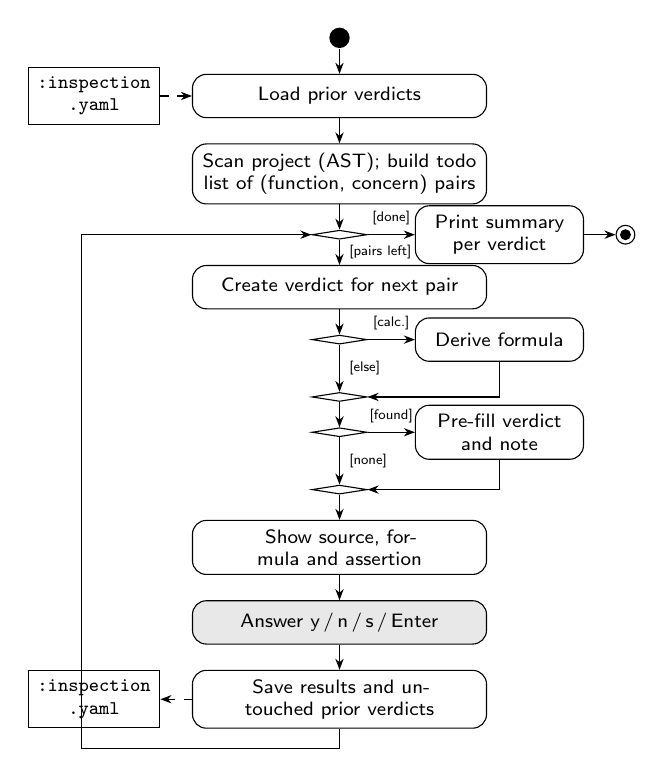
\begin{tikzpicture}[
  font=\sffamily\scriptsize, >={Stealth[length=4pt]}, node distance=3.2mm,
  act/.style={draw, rounded corners=5pt, align=center, minimum height=5.5mm, text width=3.5cm, fill=white},
  rev/.style={act, fill=gray!18},
  dec/.style={draw, diamond, aspect=1.6, inner sep=1pt, minimum width=7mm, fill=white},
  obj/.style={draw, rectangle, minimum height=5mm, align=center, font=\ttfamily\scriptsize},
  g/.style={font=\sffamily\tiny},
  every path/.style={->, thin}]
  \node[circle, fill=black, inner sep=2.6pt] (start) {};
  \node[act, below=of start] (load) {Load prior verdicts};
  \node[act, below=of load] (scan) {Scan project (AST); build todo list of (function, concern) pairs};
  \node[dec, below=of scan] (more) {};
  \node[act, below=of more] (verd) {Create verdict for next pair};
  \node[dec, below=of verd] (calc) {};
  \node[act, text width=1.9cm, right=6mm of calc] (form) {Derive formula};
  \node[dec, below=6mm of calc] (m1) {};
  \node[dec, below=of m1] (prior) {};
  \node[act, text width=1.9cm, right=6mm of prior] (pre) {Pre-fill verdict and note};
  \node[dec, below=6mm of prior] (m2) {};
  \node[act, below=of m2] (show) {Show source, formula and assertion};
  \node[rev, below=of show] (ans) {Answer y\,/\,n\,/\,s\,/\,Enter};
  \node[act, below=of ans] (save) {Save results and untouched prior verdicts};
  \node[act, text width=1.9cm, right=6mm of more] (sum) {Print summary per verdict};
  \node[circle, draw, inner sep=2.4pt, right=4mm of sum] (end) {};
  \node[circle, fill=black, inner sep=1.4pt] at (end) {};
  \node[obj, left=4mm of load] (y1) {:inspection\\.yaml};
  \node[obj, left=4mm of save] (y2) {:inspection\\.yaml};

  \draw (start) -- (load);
  \draw (load) -- (scan);
  \draw (scan) -- (more);
  \draw (more) -- node[g, right] {[pairs left]} (verd);
  \draw (more) -- node[g, above] {[done]} (sum);
  \draw (sum) -- (end);
  \draw (verd) -- (calc);
  \draw (calc) -- node[g, above] {[calc.]} (form);
  \draw (form) |- (m1);
  \draw (calc) -- node[g, right] {[else]} (m1);
  \draw (m1) -- (prior);
  \draw (prior) -- node[g, above] {[found]} (pre);
  \draw (pre) |- (m2);
  \draw (prior) -- node[g, right] {[none]} (m2);
  \draw (m2) -- (show);
  \draw (show) -- (ans);
  \draw (ans) -- (save);
  \draw (save.south) -- ++(0,-2.5mm) -| ([xshift=-14mm]save.west) |- (more.west);
  \draw[dashed] (y1) -- (load);
  \draw[dashed] (save) -- (y2);
\end{tikzpicture}
\caption{UML activity diagram of the inspection (\texttt{--inspect}). The shaded action is the reviewer's; all others are the tool's. Answers: y\,=\,accepted, n\,=\,declined, s\,=\,pending, Enter or end of input keeps the pre-filled value.}
\label{fig:inspection}
\end{figure}

\section{Design Cycles and Findings}
\emergencystretch=1.5em
\paragraph*{Cycle 1 (roles)} The first prototype (July 2026) offered decorators for the \emph{role} of a function, such as \cc{@functional}, \cc{@mapping}, \cc{@data\_input} and \cc{@data\_output}, with a checking runner and formula derivation for functional code. On the testbed, 6 of 254 functions were annotated (2\,\%), and the scan proposed 206 candidates, 113 of them as \cc{@mapping}. Nearly every function has a role, so the candidates did not tell a reviewer what to look at. A role does not name the risk.

\paragraph*{Cycle 2 (concerns)} The redesign replaced roles with concerns, each carrying an assertion, and added the inspection. On the same 254 functions with the same 6 marked, the scan finds candidates for every concern except \cc{hardware\_dependency}, from 3 for \cc{external\_tool} to 128 for \cc{mapping}. Its high-confidence rules alone yield 121 unmarked detections. The largest groups are \cc{data\_input}~(40), \cc{human\_decision}~(25), \cc{data\_output} and \cc{human\_input}~(15 each), and \cc{model\_call}~(9), followed by \cc{calculations}~(6), \cc{stochastic}~(5), \cc{external\_tool}~(3), \cc{statistical}~(2) and \cc{config}~(1). Each of these is a concrete review question. Nine unmarked model calls, for example, are nine places where a reader cannot yet tell which model version produced the data.

\paragraph*{Design principles so far}
\begin{enumerate}
\item[DP1] \emph{Name the risk, not the role.} A marker should say what could make the result untrustworthy.
\item[DP2] \emph{One assertion per concern.} The assertion is the review question; it keeps inspection short and comparable.
\item[DP3] \emph{Detect, then declare.} Static detection of unmarked places lowers the entry cost for authors who never annotate.
\item[DP4] \emph{Keep verdicts next to the code.} A versioned verdict file makes trust decisions reviewable and incremental.
\item[DP5] \emph{Keep the set open.} Concerns come from a community; adding one must be as cheap as adding a folder.
\end{enumerate}

\section{Outlook and Questions for SE Research}
Cycle~3 moves the tool into teaching: students in a master's course on responsible RSE learn the model and contribute concerns through a documented contribution path. This tests DP5 and whether people outside the designer's project find the assertions meaningful. Technically, the next step is the two runtime quadrants: fixtures that check purity and reading behaviour, and tests generated from declared formulas.

We see three questions where SE research could help. First, how precise must static detection be before authors trust its suggestions? Second, how can generated tests be derived from a declared formula and a cited method? Third, how should verdicts flow into provenance and software metadata, so that a reader of the paper sees which claims were inspected and by whom?

\bibliographystyle{IEEEtran}
\bibliography{references}

\end{document}
